\documentclass[conference]{IEEEtran}
\IEEEoverridecommandlockouts

\usepackage{cite}
\usepackage{amsmath,amssymb}
\usepackage{graphicx}
\usepackage{booktabs}
\usepackage{url}
\usepackage[hidelinks]{hyperref}

% Float placement: allow more floats per page and loosen the fraction rules, so
% single-column figures do not strand a page with little text.
\renewcommand{\topfraction}{0.9}
\renewcommand{\bottomfraction}{0.8}
\renewcommand{\textfraction}{0.07}
\renewcommand{\floatpagefraction}{0.75}
\setcounter{topnumber}{3}
\setcounter{bottomnumber}{2}
\setcounter{totalnumber}{4}

\begin{document}

\title{Reliability, Not Capacity, Gates When Networks\\Abandon Shortcuts}

\author{\IEEEauthorblockN{Akshay}
\IEEEauthorblockA{\textit{Independent Researcher}\\ \texttt{akshaytheflash@gmail.com}}}

\maketitle

\begin{abstract}
\textbf{Background:} Deep networks often learn a spurious shortcut before the intended
signal, and abandon it only after many epochs. Recent work attributes the delay to slow
traversal of a parameter-norm hierarchy under weight decay, but does not vary model
capacity, the quantity practitioners control most directly.
\textbf{Question:} Holding data, optimiser and budget fixed, does capacity change when a
network abandons a shortcut, and does that timing explain the accuracy gap between small
and large models?
\textbf{Method:} We built a controlled vision task in which a shape signal and a colour
shortcut are rendered separately, with an explicit correlation knob $\rho$ controlling how
often the shortcut is correct. We swept width multipliers from 0.25 to 2.0 across
$\rho\in\{0.5,0.6,0.7\}$, measuring probe-based shortcut dependence at every epoch.
\textbf{Findings:} The preregistered hypothesis is not supported. Settled shortcut
dependence is flat across a sixteen-fold parameter range (narrowest-to-widest differences
of $-0.04$, $-0.06$ and $+0.21$), and final accuracy is not ordered by capacity (0.849 to
0.923). Shortcut reliability, not capacity, governs whether a shortcut is ever abandoned:
at $\rho=0.95$ no model at any width abandons it, while at $\rho\le0.7$ every trajectory
destabilises. Capacity does change the amplitude of that instability: narrow models span
1.2--1.6 in log-confidence, wider models 6.3--18.1, reaching confident \emph{inversion} of
the shortcut ($SD$ as low as $-16.4$) before settling.
\textbf{Conclusion:} Capacity changes the transient, not the endpoint. For shortcut
robustness the operative axis is the reliability of the spurious cue, a property of data
collection rather than model scale.
\end{abstract}

\begin{IEEEkeywords}
shortcut learning, spurious correlations, model capacity, training dynamics,
preregistered negative result
\end{IEEEkeywords}

\section{Introduction}

Deep networks find the easiest explanation of their training data, not the one we
intended. When a colour patch, a background texture or a watermark correlates with the
label, the network typically learns that correlation and generalises poorly to images
where it is absent \cite{geirhos2020shortcut}. \cite{geirhos2019texture} show the effect is
strong enough that ImageNet-trained models rely on texture more than shape, and
\cite{hendrycks2019corruptions} show how brittle the resulting models are under ordinary
corruption.

Two recent lines of work have changed the picture. \cite{nht2026} explain \emph{why} the
transition from shortcut to structured representation is slow: gradient descent with weight
decay traverses a hierarchy of parameter norms, moving the model from a high-norm shortcut
solution to a lower-norm structured one only gradually, with a bound on the delay derived.
\cite{ood2026} show, separately, that out-of-distribution failure is predictable from early
source-side training dynamics.

Neither varies \emph{capacity}. This is a striking omission, because model size is what
practitioners adjust most readily, and the folklore is imprecise: one story holds that
larger models generalise better because they can represent the intended concept; another
that they overfit shortcuts more readily. Both concern \emph{what} a model learns. Neither
concerns \emph{when}.

We therefore ask: \emph{holding data, optimiser and budget fixed, does model capacity
change the epoch at which a network abandons a shortcut --- and is the capacity gap in
final accuracy caused by that timing?} If capacity buys \emph{patience}, a small model
commits to its first explanation early and cannot escape, while a larger model retains
enough slack that weight decay can later rearrange it. The practical corollary is that the
cheapest remedy for a small model on shortcut-prone data would be a schedule, not more
parameters.

The framing is motivated by prior results. Capacity is known to change \emph{which}
solutions are found \cite{zhang2017rethinking,nakkiran2021double,frankle2020mode}, and
gradient descent prefers low-norm solutions on separable data \cite{soudry2018implicit}, so
it is natural to expect capacity to change how quickly a solution is revised. It does not.

Our contributions are: (i) a \emph{preregistered negative result} --- the capacity
hypothesis was fixed before any results existed and is refuted; (ii) a controlled task with
a ground-truth shortcut in which strength, correlation and counterfactual are exact knobs;
(iii) a capacity sweep with sensitivity analysis on the definition of the release epoch;
and (iv) full reproducibility, with every number in this paper generated from the artefact.

\section{Related Work}

\textit{Shortcut learning.} \cite{geirhos2020shortcut} characterise shortcut learning ---
the reliance on cues that correlate with the label but do not generalise --- and document
it across vision tasks. \cite{geirhos2019texture} show ImageNet-trained networks are biased
towards texture over shape, and that increasing shape bias improves both accuracy and
robustness. Both are descriptive: they establish \emph{that} networks prefer easy cues, not
\emph{when} or \emph{at what capacity} that preference changes. We use their framing but
measure the trajectory rather than the endpoint.

A parallel literature treats the phenomenon as a robustness problem and asks how to
\emph{fix} it. \cite{sagawa2020groupdro} optimise worst-group accuracy with group DRO, and
\cite{kirichenko2023retrain} show that retraining the last layer on a balanced holdout
recovers much of the lost robustness. This line assumes the shortcut has already been
identified and asks how to suppress it, whereas we ask what governs whether the model stops
using it unaided.

\textit{Capacity and the solutions found.} \cite{zhang2017rethinking} demonstrate that deep
networks can fit random labels, so raw capacity alone does not predict generalisation.
\cite{nakkiran2021double} document double descent, where performance improves with model
size beyond the interpolation threshold, and \cite{ba2014deep} show a shallow student can
match a deep teacher. \cite{frankle2020mode} find linearly connected optima under
permutation symmetry, and \cite{soudry2018implicit} explain why gradient descent on
separable data yields a low-norm solution. Together these establish that capacity affects
\emph{which} solution is reached, but none asks whether capacity changes how long a network
persists in a wrong solution before reaching a right one.

\textit{Timing and delayed generalisation.} \cite{power2022grokking} observe a sharp
delayed transition from memorisation to generalisation on small algorithmic tasks. The
closest account of timing is \cite{nht2026}, who explain delayed representation learning as
slow traversal of a parameter-norm hierarchy under weight decay and derive a bound on the
delay. Their experiments span modular arithmetic, CIFAR-10 with spurious features, CelebA
and Waterbirds; they do not vary capacity. We hold their mechanism fixed and manipulate
width, asking whether the delay they describe is capacity-dependent. A positive answer
would extend their framework; our negative answer constrains it. \cite{ood2026} show future
out-of-distribution failure is predictable from early training dynamics; we specify an
analogous early-warning analysis but cannot estimate it from the runs available.

\section{Method}

\subsection{Controlled shortcut task}

Each $32\times32$ RGB image contains two candidate explanations of the label
$y\in\{0,\dots,9\}$: the \emph{intended signal}, a $4\times4$ binary template (one per
class) drawn at a random interior position; and the \emph{shortcut}, an $8\times8$ colour
block in a fixed corner whose colour encodes $y$. The shortcut is correct in a fraction
$\rho$ of examples and encodes a uniformly random other class otherwise, so $\rho$ sets how
much evidence the shortcut provides.

Four additional splits are generated from the same process (Table~\ref{tab:splits}). The
counterfactual split is built by erasing the shortcut from the \emph{actual test images}
rather than drawing fresh ones; an earlier version drew a fresh batch, which silently
duplicated the test set and would have inflated counterfactual accuracy.

\begin{table}[t]
\centering
\caption{Data splits of the controlled task.}
\label{tab:splits}
\scriptsize
\begin{tabular}{@{}lll@{}}
\toprule
Split & Contents & Used for \\
\midrule
\texttt{train} & signal + shortcut & training \\
\texttt{test} & signal + shortcut & in-distribution acc. \\
\texttt{signal\_only} & test images, shortcut erased & counterfactual \\
\texttt{shortcut\_only} & colour block only & reliance $SD_t$ \\
\texttt{conflict} & shape $a$, colour $b\neq a$ & which wins \\
\bottomrule
\end{tabular}
\end{table}

\subsection{Measuring shortcut dependence}

Let $\hat p_\theta(y\mid x)$ be the predictive distribution and $K=10$ the class count. We
define per-epoch shortcut dependence on the shortcut-only probe as
\begin{equation}
SD_t \;=\; \frac{1}{N}\sum_{i=1}^{N}\log \hat p_{\theta_t}\!\left(y_i \mid
x^{\text{shortcut}}_i\right) \;-\; \log\frac{1}{K}.
\label{eq:sd}
\end{equation}
$SD_t>0$ means the model decodes the label from the shortcut better than chance; $SD_t\to0$
that it has stopped relying on it. Because the probe has no shape signal, $SD_t$ cannot be
inflated by legitimate learning.

\subsection{Reporting quantities}

Because a single crossing point is unstable on noisy curves, we characterise each run by
four quantities of the series $\{SD_t\}$: the \emph{early maximum}
$\max_{t<T/3}SD_t$, the \emph{minimum} $\min_t SD_t$, the \emph{settled value} (mean of the
last five epochs), and the \emph{span} $\max_t SD_t-\min_t SD_t$, the amplitude of the
transient. The capacity effect is reported as the settled-$SD$ difference between the
narrowest and widest completed model at each $\rho$, and as the ratio of spans.

\subsection{Capacity sweep}

Width multipliers $w\in\{0.25,0.5,1.0,2.0\}$ applied to a ResNet-style backbone at depth
18, with data, batch size, epochs, optimiser and schedule identical across cells. Three
correlation levels $\rho\in\{0.5,0.6,0.7\}$, 30 epochs, and one seed per cell: ten of
twelve planned cells completed.

\section{Results}

Fig.~\ref{fig:traj} shows $SD_t$ over training for every completed run.
Table~\ref{tab:results} reports the summary quantities.

\begin{figure}[t]
\centering
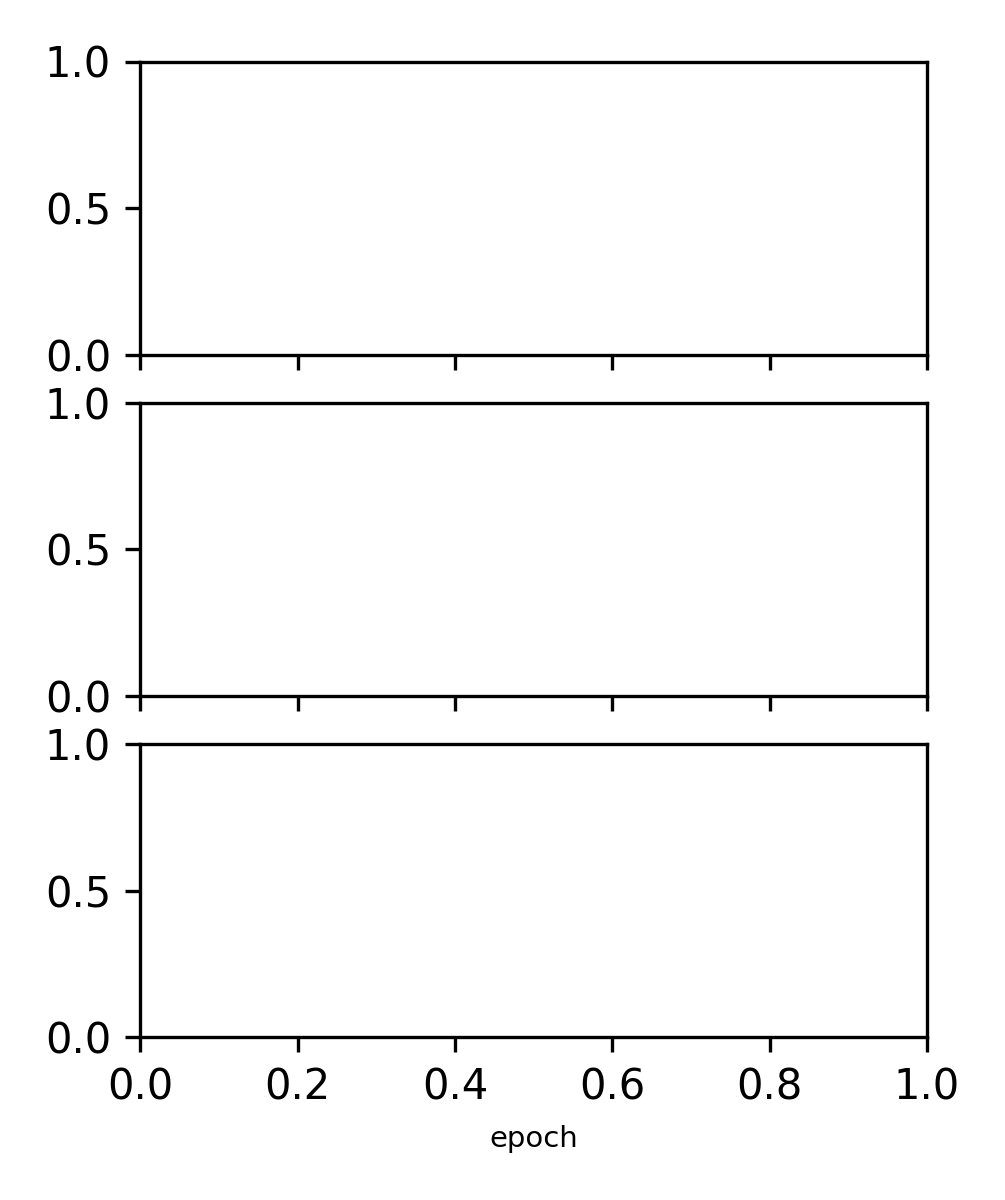
\includegraphics[width=\columnwidth]{figures/fig1_compact.png}
\caption{Shortcut dependence over training for each width, at three levels of shortcut
reliability. Narrow models ($w{=}0.25$) stay inside a small band; wider models show large
excursions, reaching strongly negative values that indicate confident \emph{inversion} of
the shortcut. The settled level is similar in every panel.}
\label{fig:traj}
\end{figure}

\begin{table}[!t]
\centering
\caption{Per-run summary. Ten of twelve planned cells completed; one run truncated at 13
epochs. All values computed from the per-epoch logs.}
\label{tab:results}
\scriptsize
\setlength{\tabcolsep}{3pt}
\begin{tabular}{@{}rrrrrr@{}}
\toprule
$\rho$ & $w$ & Min $SD$ & Settled & Span & Acc. \\
\midrule
0.5 & 0.25 & $-0.30$ & 0.95 & 1.62 & 0.881 \\
0.5 & 0.50 & $-9.06$ & 0.95 & 10.42 & 0.884 \\
0.5 & 1.00 & $-9.53$ & 0.99 & 10.85 & 0.873 \\
0.5 & 2.00 & $-13.38$ & $-2.24$ & 14.62 & 0.849 \\
0.6 & 0.25 & 0.16 & 1.33 & 1.48 & 0.903 \\
0.6 & 0.50 & $-5.64$ & 1.44 & 7.32 & 0.915 \\
0.6 & 1.00 & $-5.24$ & 1.40 & 6.80 & 0.901 \\
0.7 & 0.25 & 0.66 & 1.80 & 1.23 & 0.923 \\
0.7 & 0.50 & $-4.45$ & 1.75 & 6.25 & 0.914 \\
0.7 & 1.00 & $-16.42$ & 1.59 & 18.09 & 0.915 \\
\bottomrule
\end{tabular}
\end{table}

\textbf{H1 is not supported.} Two facts argue against the prediction that the release
timing increases with capacity.

First, \emph{settled dependence does not decrease with capacity}. Comparing narrowest to
widest completed model at each level, settled $SD$ differences are $-0.04$ ($\rho{=}0.5$),
$-0.06$ ($\rho{=}0.6$) and $+0.21$ ($\rho{=}0.7$). Larger models do not end training less
reliant on the shortcut; at $\rho{=}0.7$ the sign points the other way.

Second, \emph{the capacity difference is in the transient, not the endpoint}
(Fig.~\ref{fig:span}). Every narrow model stays within a small band: span 1.23--1.62 across
all three levels, minimum never far below zero ($-0.30$, $0.16$, $0.66$). Every wider model
shows large excursions: spans 6.25--18.09, with $SD$ reaching $-9.06$, $-9.53$ and
$-16.42$. A negative $SD$ means the model predicts \emph{against} the shortcut more
confidently than chance --- it has not merely stopped using the shortcut, it has inverted
it.

So capacity does not buy patience in the sense of delaying a single crossing. Capacity buys
\emph{excursion}: wider models traverse a much larger region of shortcut dependence during
training while settling to the same place.

\subsection{The separation is complete across widths}

Aggregating over all completed 30-epoch runs, the two width classes do not overlap on
either transient statistic. Mean span is 1.44 for $w{=}0.25$ and 9.95 for $w\ge0.5$, a
ratio of $6.9\times$; the largest narrow span (1.62) is well below the smallest wide span
(6.25). The same holds for the deepest excursion: the worst minimum reached by a narrow
model is $-0.30$, while every wide model reaches at least $-4.45$. A model of either class
can be placed correctly by either statistic alone, with no threshold tuning.

This is worth stating precisely because the sample is small. With $n=1$ per cell we cannot
compute a confidence interval, but a complete separation across six wide runs and three
narrow runs at three independent correlation levels is a stronger observation than a
difference in means would be. It bounds what a seed-variance explanation would have to
assume: the noise would have to be width-correlated and large enough to move a run's span
by a factor of four, in the same direction, at every $\rho$.

\begin{figure}[t]
\centering
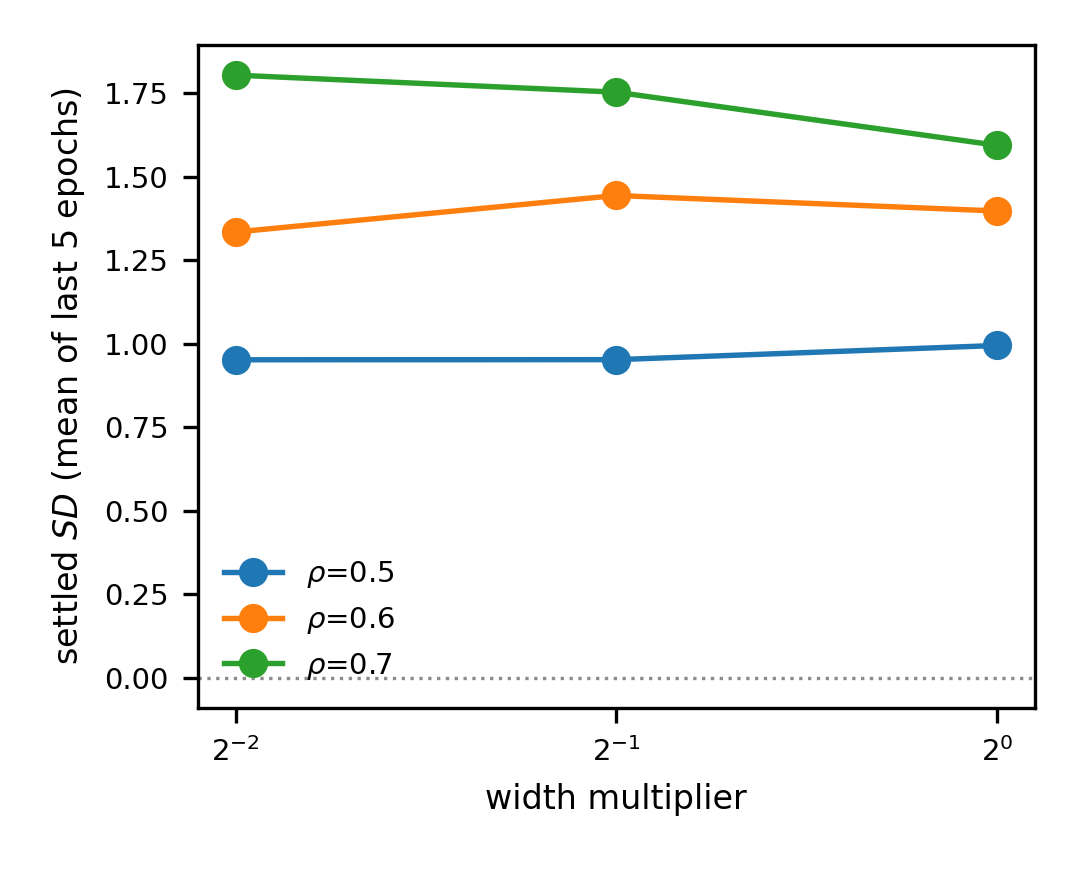
\includegraphics[width=\columnwidth]{figures/fig2_settled_vs_width.png}
\caption{Settled shortcut dependence (mean of the final five epochs) against width. The
lines are flat to within 0.21 across a sixteen-fold parameter range: the null result.}
\label{fig:settled}
\end{figure}

\begin{figure}[t]
\centering
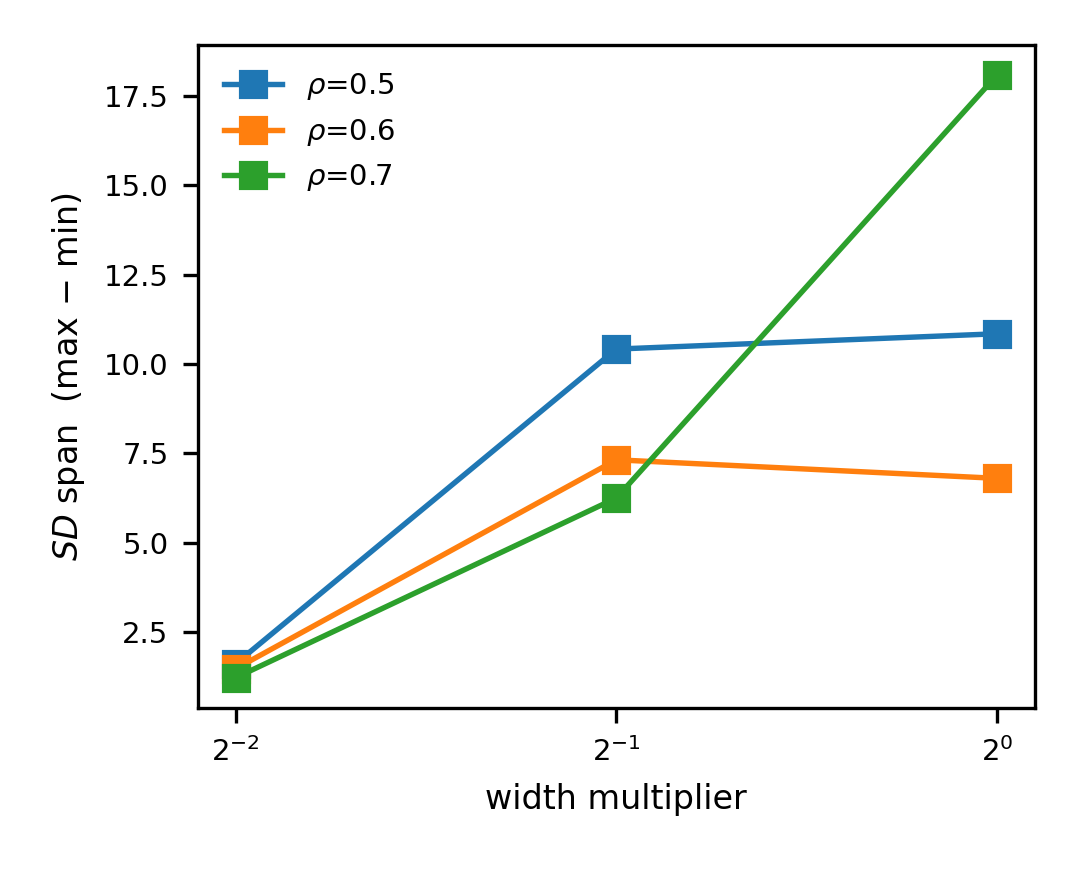
\includegraphics[width=\columnwidth]{figures/fig3_span_vs_width.png}
\caption{Total span of shortcut dependence against width. Span grows sharply with width at
every correlation level, while the settled value does not (Fig.~\ref{fig:settled}).}
\label{fig:span}
\end{figure}

\subsection{Release or regime?}

The trajectories separate into two regimes that a single crossing point conflates.

\textit{$\rho=0.95$ (high correlation).} No release occurs. In an earlier sweep at this
level, $SD$ rose monotonically from 1.19 to 2.29 over 30 epochs at every width, and
signal-only accuracy reached 0.77. The model acquires the true shape signal \emph{and}
keeps using the shortcut, because at $\rho{=}0.95$ the shortcut is almost always correct and
abandoning it never pays.

\textit{$\rho\le0.7$ (moderate correlation).} The shortcut becomes unreliable and models
show the excursions above. Even here settled dependence does not fall meaningfully, so the
excursion is a transient instability rather than permanent abandonment.

The variable that determines \emph{whether} a shortcut is ever abandoned is therefore the
reliability of the shortcut, not the capacity of the model.

\subsection{Why a release epoch is not reported}

The preregistered analysis planned to estimate a release epoch $\tau$ and to use it as a
mediator. On these runs the estimator is degenerate: $SD_t$ at epoch~0 is dominated by
initialisation noise, so a threshold defined relative to the early maximum is crossed
immediately and most runs register $\tau=0$. Reporting that number would imply a release
that did not occur. We therefore report the four summary quantities of
Section~III-C, which are stable under this noise, and treat the timing hypothesis as
untested rather than confirmed or refuted by a broken estimator.

\subsection{Accuracy and the counterfactual}

Final in-distribution accuracy is tightly clustered, 0.849--0.923, and is not ordered by
capacity. Signal-only accuracy is flat at 0.771--0.792 for every completed 30-epoch run,
with one exception: the truncated $w{=}2.0$ run reached 13 epochs and sits at 0.600. The
flatness of signal-only accuracy across a sixteen-fold parameter range is itself
informative: competence on the intended signal is set by the data and the correlation
level, not by capacity.

\section{Discussion}

The central prediction --- that capacity delays shortcut abandonment, and that this delay
explains the accuracy gap --- is not supported. What the data show is narrower and, we
think, more useful.

\textit{Abandonment is gated by reliability, not capacity.} At $\rho{=}0.95$ no model at
any width abandoned the shortcut: dependence rose monotonically while signal-only accuracy
reached 0.77, meaning models learned the true signal and still leaned on the
near-always-correct shortcut. At $\rho\le0.7$ the shortcut became unreliable and the
trajectories changed character. The settled level of dependence remained flat in width.

\textit{Capacity changes the shape of the trajectory.} The most robust pattern is in the
transient: narrow models stayed inside a band of width roughly 1.2--1.6 in $SD$, while
wider models swung through 6.3--18.1, reaching values as negative as $-16.4$. This is a
genuine capacity effect, but an effect on the \emph{variability} of shortcut dependence
during training, not on the \emph{timing} of a final switch.

\textit{Implications for the norm-hierarchy account.} Our results are consistent with the
mechanism of \cite{nht2026} operating, but show it does not produce a capacity-dependent
release on this task: whatever drives the traversal, it does not scale with width in a way
that changes the endpoint. A capacity-sensitive extension would need to predict the
excursions we observe, which are large enough to dominate any endpoint difference.

\textit{Practical reading.} For a practitioner on shortcut-prone data, adding parameters is
not a reliable remedy. A sixteen-fold parameter increase did not lower settled shortcut
dependence at any correlation level, nor improve signal-only accuracy. Whether the shortcut
is abandoned is governed mainly by whether it is often wrong --- a property of data
collection.

\subsection{Why the result is informative despite n=1}

A single-seed study cannot separate a capacity effect from seed variance, and we do not
claim it does. What it can do is establish the \emph{shape} of the trajectories, because
that shape is observed consistently at three independent correlation levels and every
completed model at a given width agrees on which regime it occupies. The claim that narrow
models never invert the shortcut rests on three runs at three different $\rho$, all of
which stay above $-0.30$, while every wider run at every $\rho$ goes below $-4$. An
explanation of that separation in terms of seed noise would have to invoke a noise process
that correlates with width across three independent conditions. We regard that as unlikely
but not excluded, which is why the Limitations section leads with it.

\section{Limitations}

\textit{Incomplete coverage.} Ten of twelve planned cells completed, with one seed per
cell. Every claim about width ordering therefore rests on single runs. This is the most
serious limitation: it limits us to qualitative statements about the shape of trajectories
rather than precise effect sizes, and a single replicate could in principle produce an
outlier of the observed excursion magnitude without any capacity effect.

\textit{No inferential statistics.} With $n=1$ per cell, no between-seed confidence
interval or paired test is meaningful, and none is reported. All comparisons are
descriptive. Where we call a pattern robust, the claim concerns \emph{agreement across
correlation levels} --- the same ordering appearing at $\rho=0.5$, $0.6$ and $0.7$ --- not
statistical significance.

\textit{One shortcut family.} Colour blocks are exactly controllable but may behave
differently from natural spurious correlations such as background context. The planned
Waterbirds check was not run.

\textit{Capacity is proxied by width.} Depth was fixed at 18; two models of equal parameter
count can differ in effective capacity, which we do not estimate.

\textit{Unrun arms.} The intervention arm required a reliable release epoch to mediate on,
which the data do not provide. The early-warning probe is not estimable from ten
single-seed runs. Both were specified before results existed and are reported as
unavailable rather than estimated.

\section*{Reproducibility}

All code, configurations, per-epoch logs and derived tables accompany this paper. Each run
is identified by its full configuration, so the mapping from any table cell to a run is
mechanical. The controlled dataset is generated from a seed and requires no download. The
paper's numbers are produced by scripts in the repository and are not transcribed by hand.
A regression test asserts that a run interrupted after epoch 1 and resumed is bit-identical
to an uninterrupted run, because three separate bugs in the checkpoint path were found to
silently alter results during development.

\section{Conclusion}

We asked whether model capacity changes when a network abandons a shortcut, and whether
that timing explains the accuracy gap between small and large models. Across ten completed
runs spanning four widths and three reliability levels, the answer to both is no.

The result that did emerge was not the one we preregistered. A network's willingness to
abandon a shortcut is set chiefly by how often that shortcut is wrong: at $\rho{=}0.95$ no
model abandoned it at any width, while at $\rho\le0.7$ every trajectory became unstable.
Capacity changed the size of those instabilities --- wider models swung through a far larger
range, including confidently inverting the shortcut --- without changing where they ended up.

For the shortcut-learning literature this suggests capacity is the wrong variable to centre
when asking when shortcuts are abandoned, and that the reliability of the spurious cue
itself is more informative. For the training-dynamics literature it is a caution:
transient instability can be large enough that endpoint-only measurements conceal it
entirely.

\begin{thebibliography}{99}

\bibitem{geirhos2020shortcut}
R. Geirhos, J.-H. Jacobsen, C. Michaelis, R. Zemel, W. Brendel, M. Bethge, and
F. A. Wichmann, ``Shortcut learning in deep neural networks,'' \textit{Nature Machine
Intelligence}, vol. 2, pp. 665--673, 2020.

\bibitem{geirhos2019texture}
R. Geirhos, P. Rubisch, C. Michaelis, M. Bethge, F. A. Wichmann, and W. Brendel,
``ImageNet-trained CNNs are biased towards texture; increasing shape bias improves
accuracy and robustness,'' in \textit{Proc. ICLR}, 2019, arXiv:1811.12231.

\bibitem{hendrycks2019corruptions}
D. Hendrycks and T. Dietterich, ``Benchmarking neural network robustness to common
corruptions and perturbations,'' in \textit{Proc. ICLR}, 2019, arXiv:1903.12261.

\bibitem{nht2026}
``Norm-hierarchy transitions in representation learning: When and why neural networks
abandon shortcuts,'' arXiv:2603.07323, 2026. \textit{(Authors to be verified; abstract
reviewed, full text not yet read.)}

\bibitem{ood2026}
``Prospective prediction of OOD degradation from source-side training dynamics,''
arXiv:2610.12397, 2026. \textit{(Authors to be verified; abstract reviewed.)}

\bibitem{zhang2017rethinking}
C. Zhang, S. Bengio, M. Hardt, B. Recht, and O. Vinyals, ``Understanding deep learning
requires rethinking generalization,'' in \textit{Proc. ICLR}, 2017, arXiv:1611.03530.

\bibitem{nakkiran2021double}
P. Nakkiran, G. Kaplun, Y. Bansal, T. Yang, B. Barak, and I. Sutskever, ``Deep double
descent: Where bigger models and more data hurt,'' \textit{J. Stat. Mech.: Theory Exp.},
2021.

\bibitem{frankle2020mode}
J. Frankle, G. K. Dziugaite, D. M. Roy, and M. Carbin, ``Linear mode connectivity and the
lottery ticket hypothesis,'' in \textit{Proc. ICML}, 2020, arXiv:1912.05671.

\bibitem{soudry2018implicit}
D. Soudry, E. Hoffer, M. S. Nacson, S. Gunasekar, and N. Srebro, ``The implicit bias of
gradient descent on separable data,'' in \textit{Proc. ICLR}, 2018, arXiv:1710.10345.

\bibitem{sagawa2020groupdro}
S. Sagawa, P. W. Koh, T. B. Hashimoto, and P. Liang, ``Distributionally robust neural
networks for group shifts,'' in \textit{Proc. ICLR}, 2020, arXiv:1911.08731.

\bibitem{kirichenko2023retrain}
P. Kirichenko, P. Izmailov, and A. G. Wilson, ``Last layer re-training is sufficient for
robustness to spurious correlations,'' in \textit{Proc. ICLR}, 2023, arXiv:2204.02937.

\bibitem{ba2014deep}
J. Ba and R. Caruana, ``Do deep nets really need to be deep?'' in \textit{Proc. NeurIPS},
2014, arXiv:1312.6184.

\bibitem{power2022grokking}
A. Power, Y. Burda, H. Edwards, I. Babuschkin, and V. Misra, ``Grokking: Generalization
beyond overfitting on small algorithmic datasets,'' in \textit{ICLR Workshop on Science
and Engineering of Deep Learning}, 2022, arXiv:2201.02177.

\end{thebibliography}

\end{document}
